\documentclass[11pt, a4paper]{article}

\usepackage{graphicx}
\usepackage[english]{babel}
\usepackage[utf8x]{inputenc}
\usepackage{amsmath}
\usepackage[a4paper,top=3cm,bottom=2cm,left=2cm,right=2cm,marginparwidth=1.75cm]{geometry}
\usepackage{amssymb}
\usepackage{subfig}

\graphicspath{ {./images} }
\newcommand*{\rad}{\ensuremath{\,\text{rad}}}

\makeatletter
\renewcommand*\env@matrix[1][*\c@MaxMatrixCols c]{%
  \hskip -\arraycolsep
  \let\@ifnextchar\new@ifnextchar
  \array{#1}}
\makeatother

% \begin{figure}[h]
%   \centering
%   \subfloat[caption 1]{{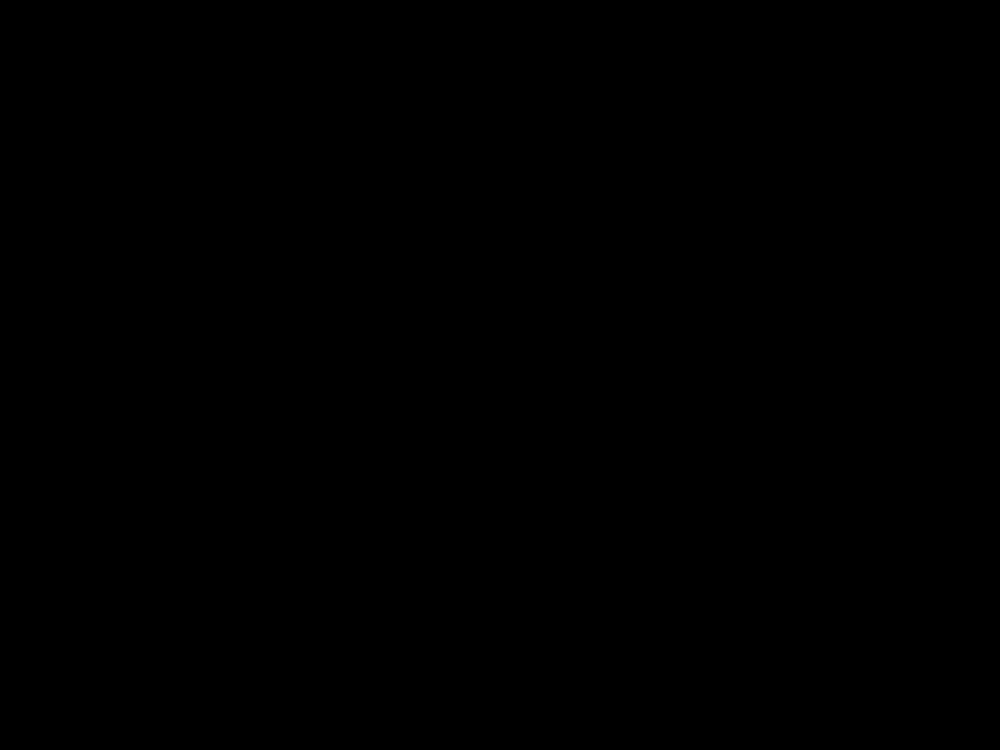
\includegraphics[width=30mm]{images/placeholder.png}}}%
%   \qquad
%   \subfloat[caption 2]{{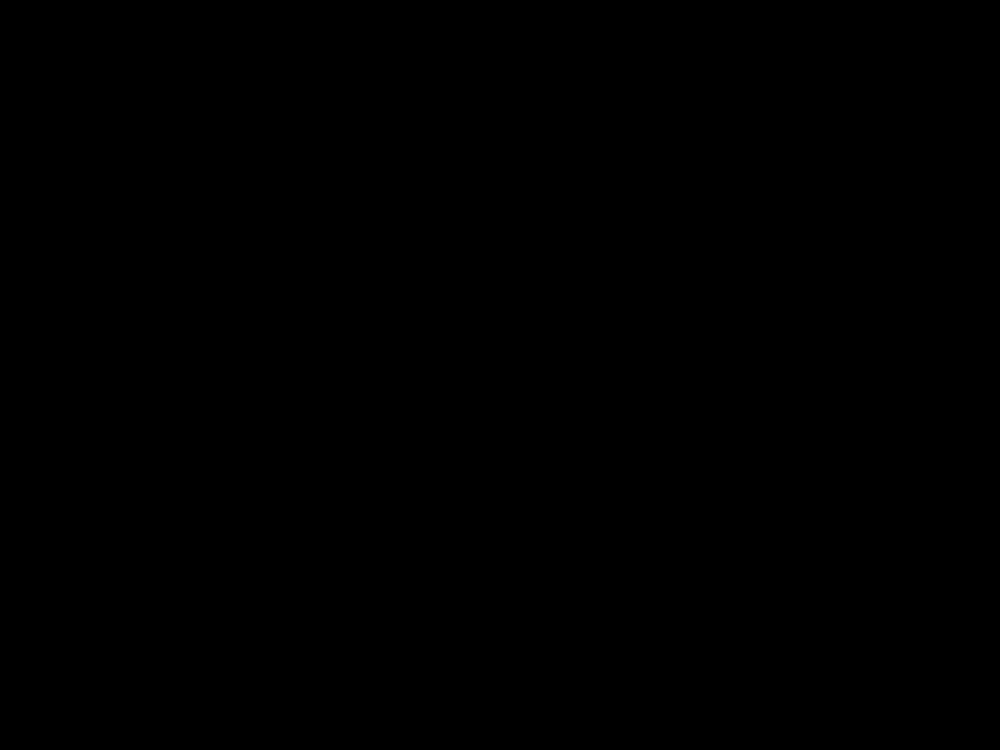
\includegraphics[width=30mm]{images/placeholder.png}}}%
%   \caption{Description}
% \end{figure}

% \begin{figure}[h]
%   \centerline{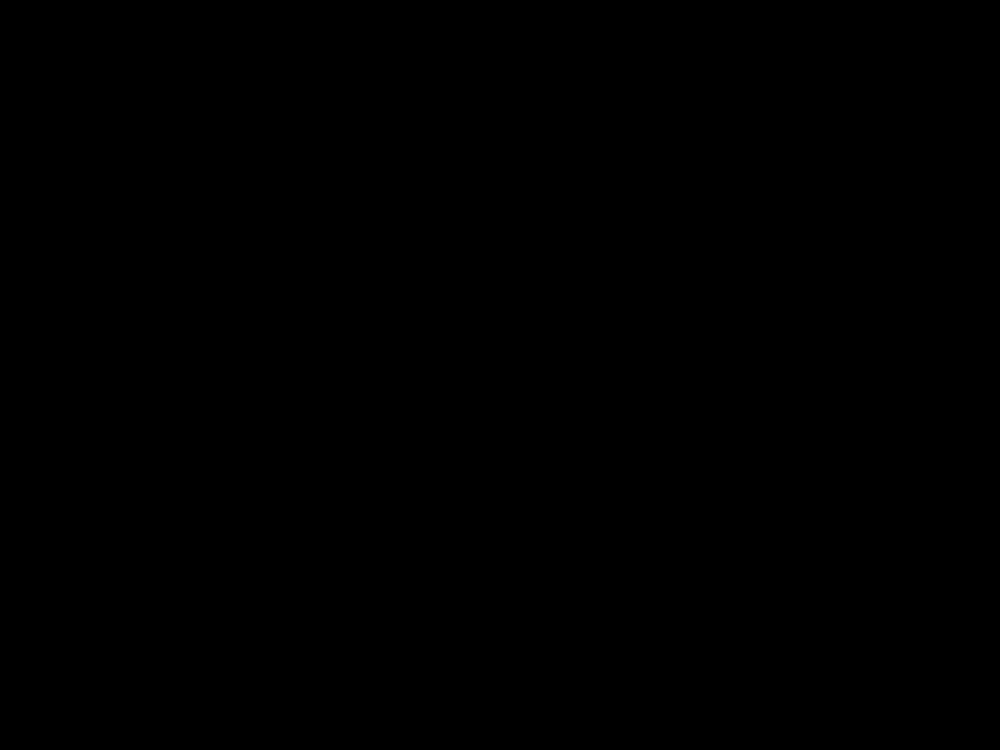
\includegraphics[width=50mm]{images/placeholder.png}}
%   \caption{Description}
% \end{figure}


\begin{document}

\setcounter{section}{11}
\section{Lecture 12 (19/03/2020)}
\subsection{Instantaneous center of zero velocity}
The Instantaneous center of zero velocity, also referred to as the instantenous center of rotation, refers to the idea that any rigid body moving on a 2D plane will have exactly 1 point with an effective instantenous velocity of 0 at a given point in time.
\begin{figure}[h]
  \centering
  \subfloat[Moving wheel]{{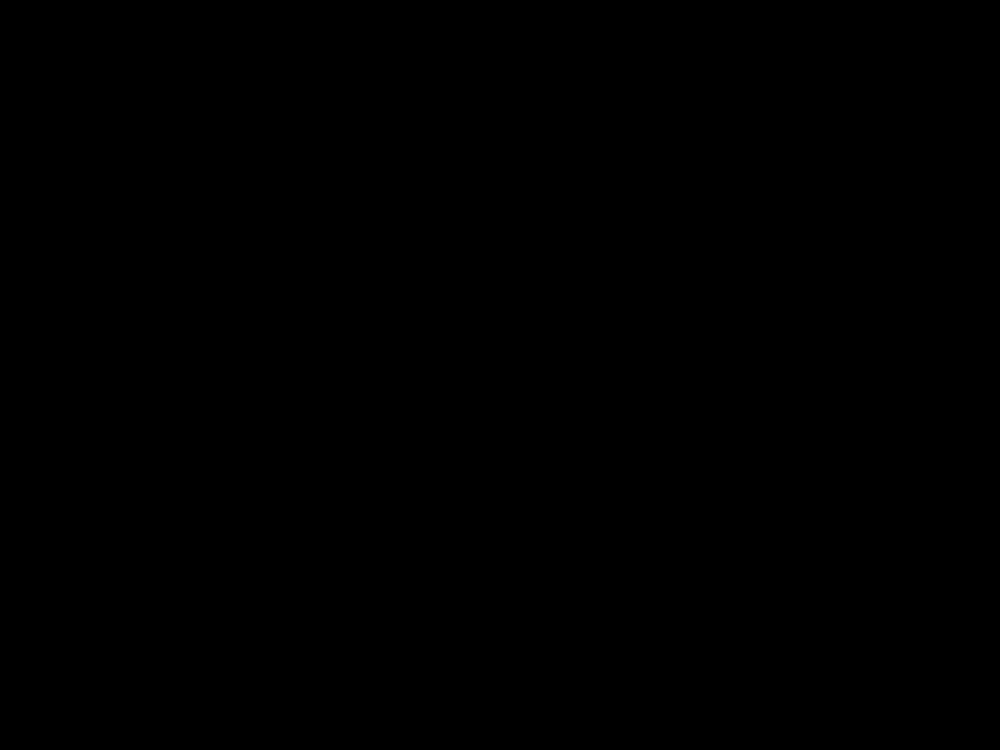
\includegraphics[width=30mm]{images/placeholder.png}}}%
  \qquad
  \subfloat[Moving bar]{{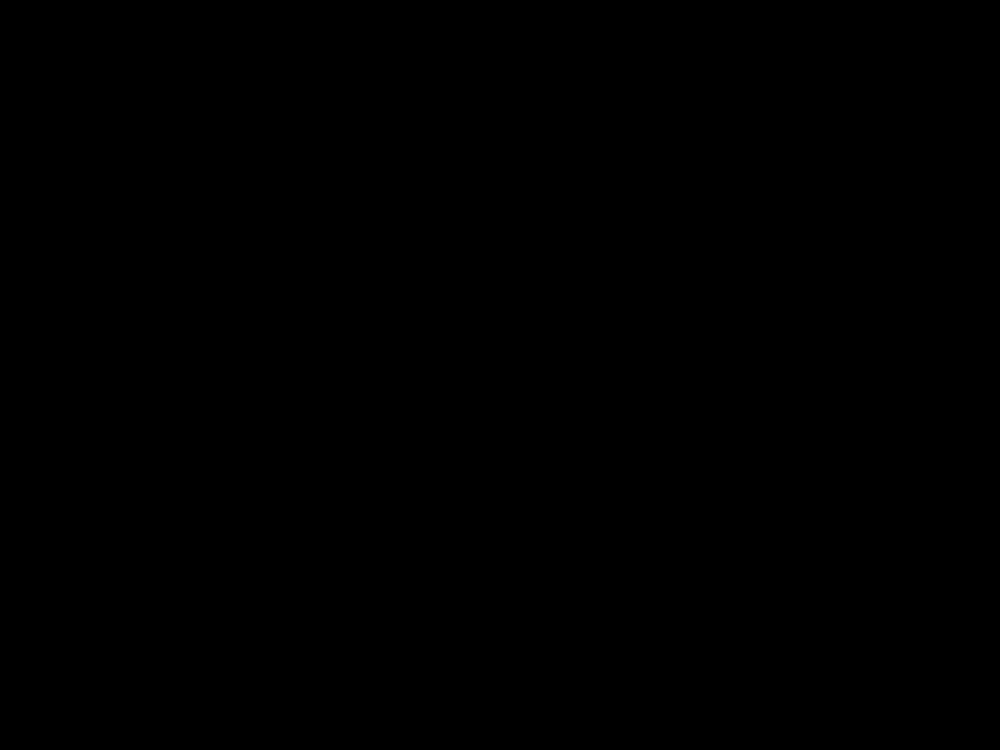
\includegraphics[width=30mm]{images/placeholder.png}}}%
  \caption{Note that the instantenous center of velocity for a wheel is it's contact point with the ground. The bar can be thought of as rotating about the instantenous center of rotation.}
\end{figure}
The IC is in fact not a single unchaniging point, but rather a point that changes over time relative to the motion. It's also important to remember that eventhough the point does not have an instantenous velocity, this does not at all imply that is also has no instantenous acceleration.

\subsection{Analysis of relative motion (velocity)}
Side note: the problems analyzing absolute motion where sometimes done using trignometry. From this point forward only vector analysis will be used since it simplifies the math and removes oppurtunities for making mistakes.\\
\\
\begin{figure}[h]
  \centering
  \subfloat[absolute frame of reference]{{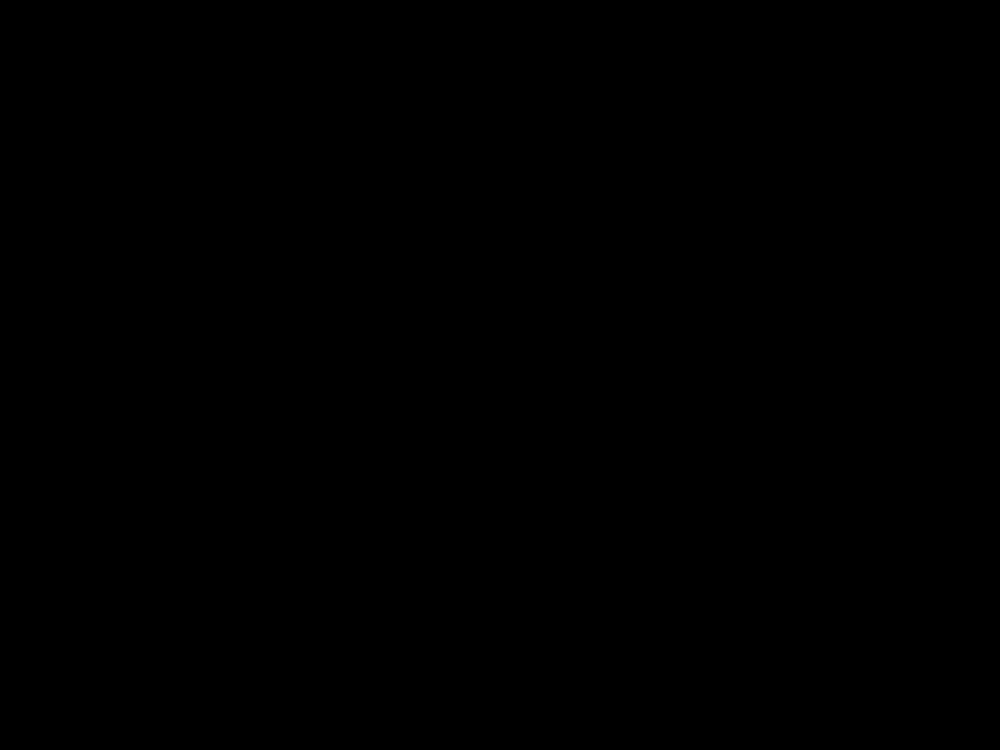
\includegraphics[width=30mm]{images/placeholder.png}}}%
  \qquad
  \subfloat[frame of reference for $B$ relative to $A$]{{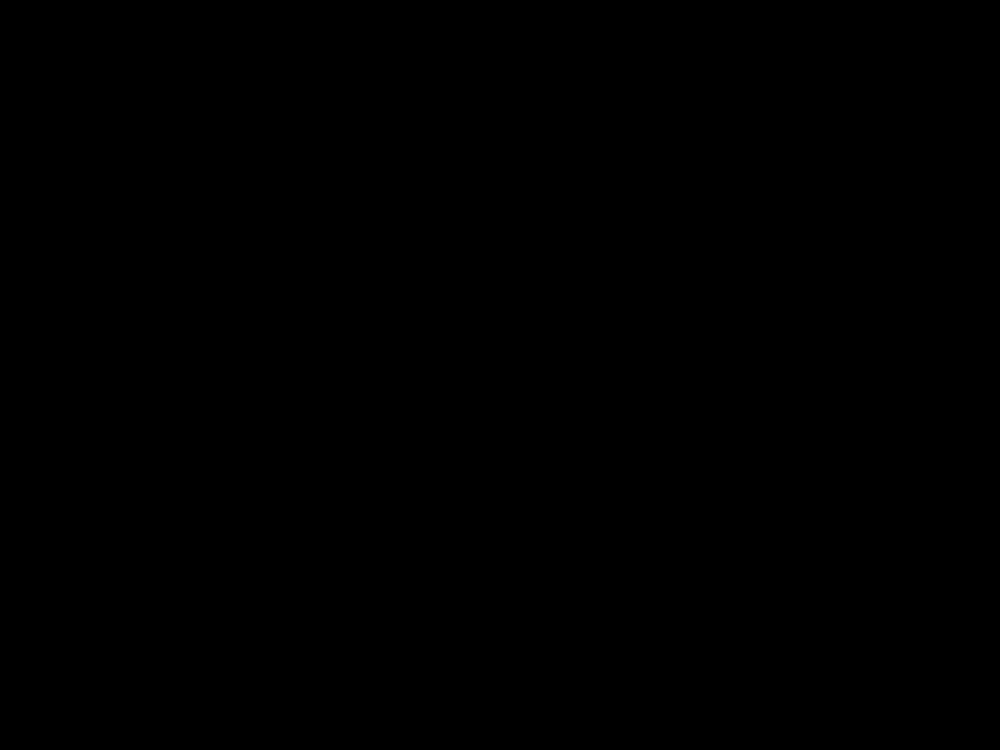
\includegraphics[width=30mm]{images/placeholder.png}}}%
  \caption{The difference between analyzing the absolute motion of $B$ and the motion of $B$ with respect to $A$}
\end{figure}
The relative position of $B$ can be described as:
\begin{gather}
  \vec{r}_B = \vec{r}_A + \vec{r}_{B/A}\\
  \begin{bmatrix} r_{Bx}\\ r_{By}\\ \end{bmatrix} = \begin{bmatrix} r_{Ax}\\ r_{Ay}\\ \end{bmatrix} + \begin{bmatrix} L\cos(\theta)\\ L\sin(\theta)\\ \end{bmatrix} 
\end{gather}
The velocity is then found by taking the time derrivative of equation (1):
\begin{gather}
  \vec{\dot{r}}_B = \vec{\dot{r}}_A + \vec{\dot{r}}_{B/A}
\end{gather}
$|v_B|=L\omega$ but takes alot of trig to figure out, using vectors simplifies this math.
\begin{figure}[h]
  \centerline{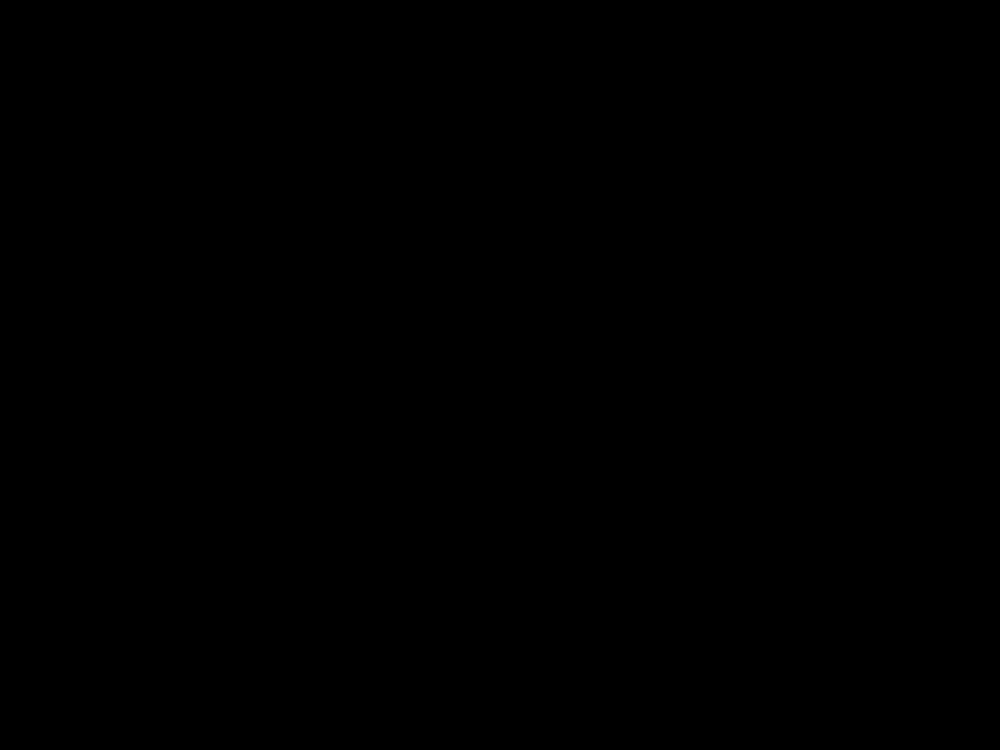
\includegraphics[width=50mm]{images/placeholder.png}}
  \caption{Description}
\end{figure}
\begin{equation}
  \omega = \begin{bmatrix} 0\\ 0\\ \omega_z\\ \end{bmatrix},\, \vec{r}_{B/A} = \begin{bmatrix} L\cos(\theta)\\ L\sin(\theta)\\ 0\\ \end{bmatrix}
\end{equation}
then:
\begin{align}
  \vec{\dot{r}}_{B/A} &= \vec{\omega} \times \vec{r}_{B/A}\\
                      &=  \begin{bmatrix} 0\\ 0\\ \omega_z\\ \end{bmatrix} \times \begin{bmatrix} L\cos  (\theta)\\ L\sin(\theta)\\ 0\\ \end{bmatrix}\\
                      &=  \begin{bmatrix} -L\omega \sin(\theta)\\ L\omega \cos(\theta)\\ 0\\ \end{bmatrix} 
\end{align}
\begin{align}
  |\vec{\dot{r}}_{B/A}| &= \sqrt{\omega^2L^2\sin^2(\theta) + \omega^2L^2\cos^2(\theta)}\\
                        &= \sqrt{\omega^2L^2} = \omega L
\end{align}
Thus the most important take-away from this is:
\begin{gather}
  \vec{v}_B = \vec{v}_A + \vec{v}_{B/A} \qquad \vec{v}_{B/A} = \vec{\omega} \times \vec{r}_{B/A}\\
  \vec{v}_B = \vec{v}_A + \vec{\omega} \times \vec{r}_{B/A}
\end{gather}

\subsection{Analysis of relative motion (acceleration)}
For acceleration a systematic vector mechanics method will also be used. Taking equation (11) and taking the time derrivative and applying the product rule:
\begin{gather}
  \vec{\dot{v}}_B = \vec{\dot{v}}_A + \vec{\dot{\omega}} \times \vec{r}_{B/A} + \vec{\omega} \times \vec{\dot{r}}_{A/B}\\
  \vec{a}_B = \vec{a}_A + \vec{\alpha} \times \vec{r}_{B/A} + \vec{\omega} \times (\vec{\omega} \times \vec{r}_{B/A})
\end{gather}
\begin{figure}[h]
  \centerline{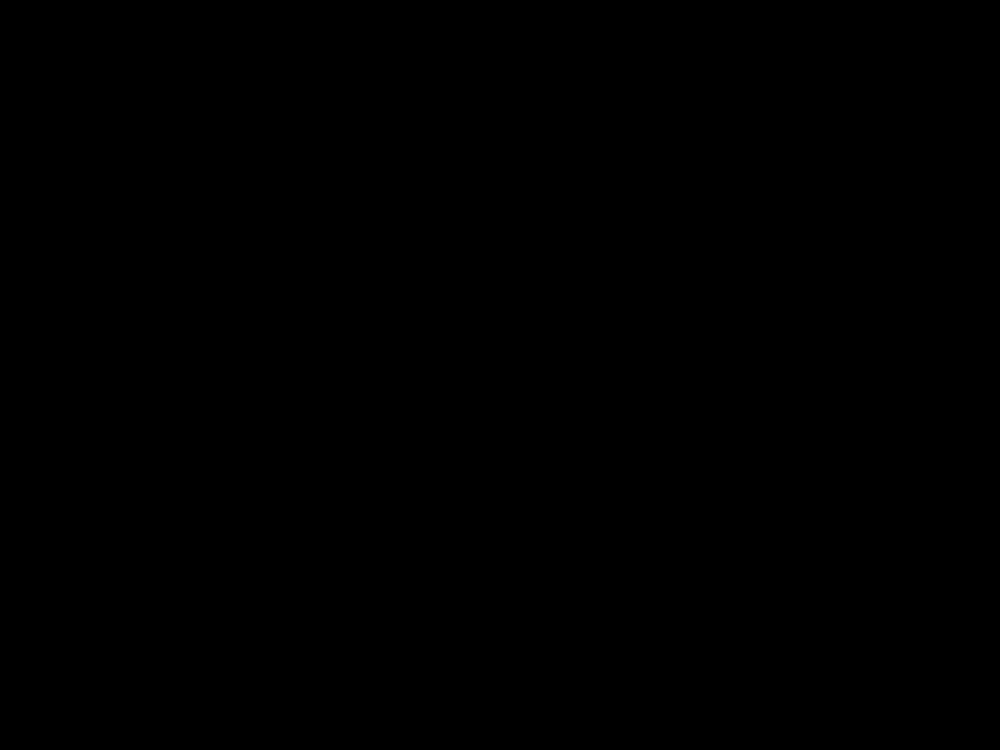
\includegraphics[width=50mm]{images/placeholder.png}}
  \caption{Visual representation of the geometry of equation (13).}
\end{figure}
Looking at figure 4 the direction of $\vec{\omega} \times (\vec{\omega} \times \vec{r}_{A/B})$ is the same direction as $\vec{r}_{B/A}$. This means that the term $\vec{\omega} \times (\vec{\omega} \times \vec{r}_{A/B}) = -\omega^2\vec{r}_{B/A}$ where $\omega$ is just a scalar. This gives the following equation:
\begin{equation}
  \vec{a}_B = \vec{a}_B + \vec{\alpha} \times \vec{r}_{B/A} - \omega^2\vec{r}_{B/A}
\end{equation}
It's very important to note that $\vec{a}_B = \vec{a}_A + \vec{\alpha} \times \vec{r}_{B/A} + \vec{\omega} \times (\vec{\omega} \times \vec{r}_{B/A})$ is the most general form of the equation. The case where $\vec{a}_B = \vec{a}_B + \vec{\alpha} \times \vec{r}_{B/A} - \omega^2\vec{r}_{B/A}$ only really holds in the special situation where $\vec{r}_{B/A}$ and $\vec{\omega}$ are \underline{orthogonal}!

\subsection{The coriolis-effect}
Important note about rotating frames of reference: The angular velocity with which the frame of reference itself is rotating will be denoted as $\Omega$ and the acceleration of the rotation of the frame of reference will be denoted as $\dot{\Omega}$.\\
\\
The coriolis-effect is an interesting effect which can be observed when objects are observed from a rotating frame of reference. In this case object which would go in a straight line when observed from a stationary frame of reference will appear to trace a curved path when observed from a rotating frame of reference. This is a very important effect for any larger scale calculation in say for example meteorolgy. This is because all motion take to be absolute on a smaller scale is in fact measured with respect to the earth which in itself is a mass rotating with the angular velocity $\Omega_{earth} = 7.272(10)^{-5} \rad/s$. Stating that motion is absolute is a good enough approximation but this doesn't hold in larger systems.
\begin{figure}[h]
  \centering
  \subfloat[$\vec{v}_B = \vec{v}_A + \vec{\omega} \times \vec{r}_{B/A}$]{{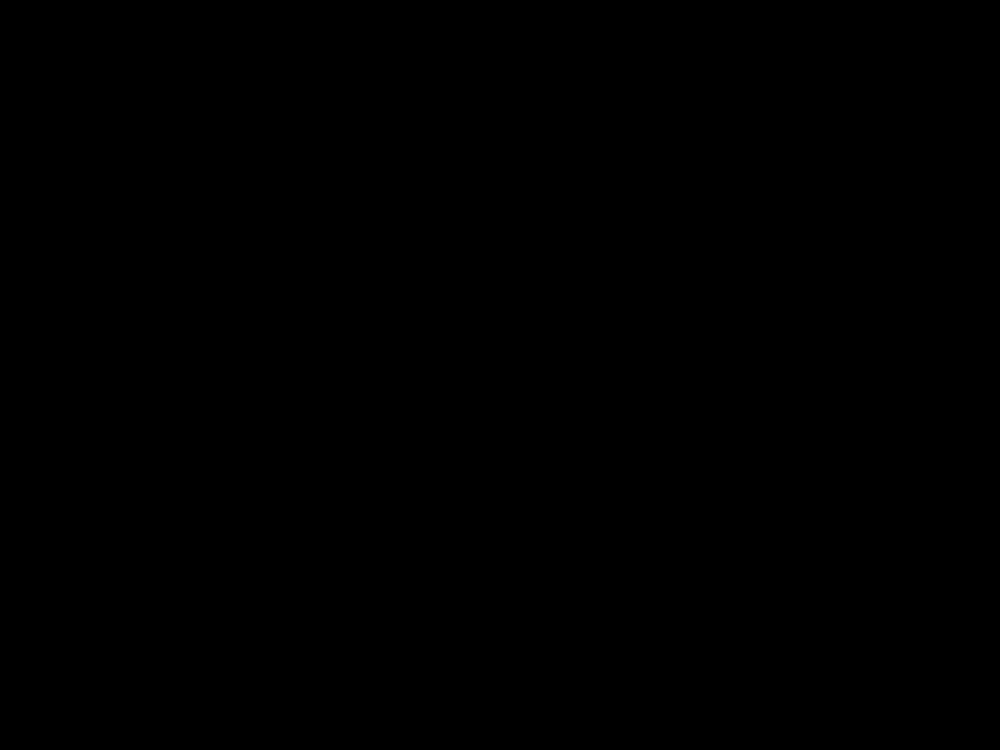
\includegraphics[width=50mm]{images/placeholder.png}}}%
  \qquad \qquad \qquad
  \subfloat[$\vec{v}_B = \vec{v}_A + \vec{\omega} \times \vec{r}_{B/A} + (\vec{v}_{B/A})_{xyz}$]{{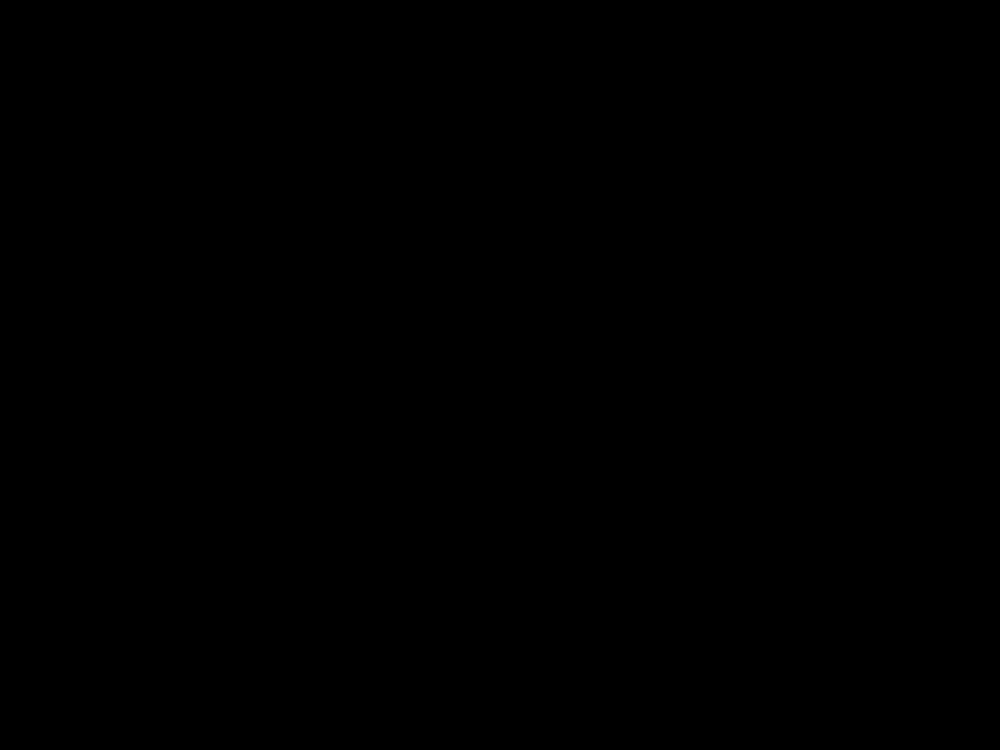
\includegraphics[width=50mm]{images/placeholder.png}}}%
  \caption{The absolute motion of $B$ in (a) and the relative motion of $B$ with respect to $A$ in (b)}
\end{figure}
the $xyz$-axis represent the frame of reference which is rotating along with $A$ with the angular velocity of $\Omega$. $XYZ$-axis represent the coordinates for absolute motion.\\
\\
Very small example involving a rotating frame of reference:
\begin{figure}[]
  \centerline{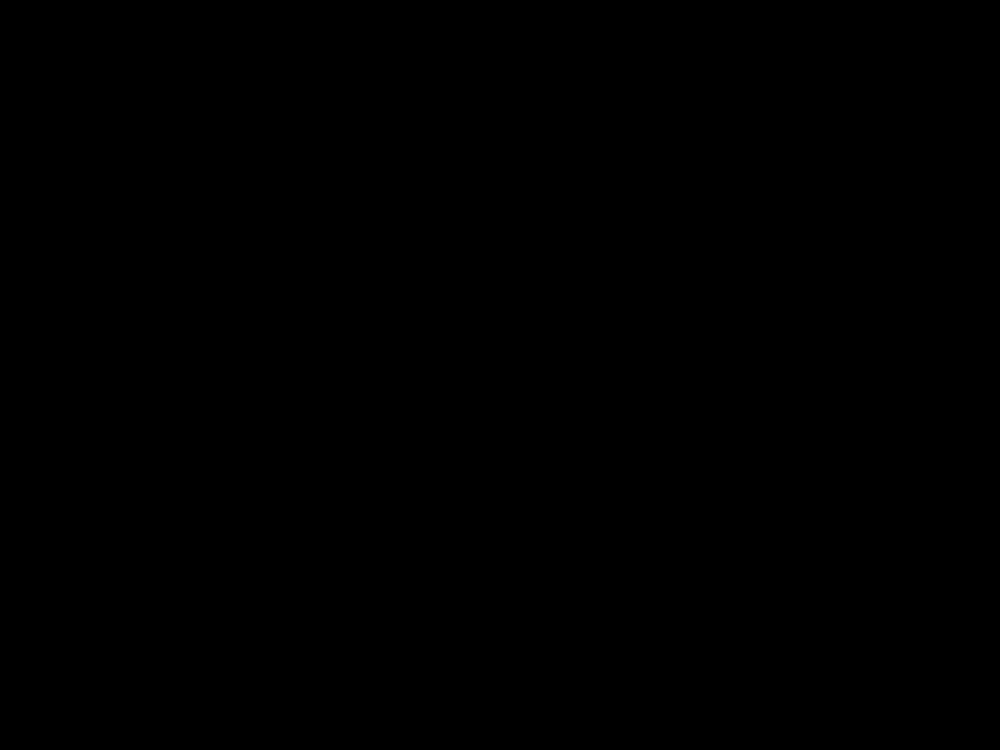
\includegraphics[width=30mm]{images/placeholder.png}}
  \caption{The relative motion of $\vec{v}_{B/A}$ where the axis $xyz$ rotate along with point $A$.0}
\end{figure}
\begin{equation}
  (\vec{v}_{B/A})_{xyz} = 
  \begin{bmatrix}
    |(\vec{v}_{B/A})_{xyz}|\cos(\phi)\\
    |(\vec{v}_{B/A})_{xyz}|\sin(\phi)\\
    0\\
  \end{bmatrix}
\end{equation}\\
\\
Thus:\\
The absolute motion of the rigid body of $AB$ is described as:
\begin{gather}
  \vec{v}_B = \vec{v}_A + \vec{\omega} \times \vec{r}_{B/A}\\
  \text{Where } \vec{\omega} \times \vec{r}_{B/A} = \vec{v}_{B/A} \notag
\end{gather}
The relative motion of $AB$ with rotating axis $xyz$ is described as:
\begin{gather}
  \vec{v}_B = \vec{v}_A + \vec{\Omega} \times \vec{r}_{B/A} + (\vec{v}_{B/A})_{xyz}\\
  \text{Where } \vec{\Omega} \times \vec{r}_{B/A} + (\vec{v}_{B/A})_{xyz} = \vec{v}_{B/A} \notag
\end{gather}
\begin{figure}[h]
  \centerline{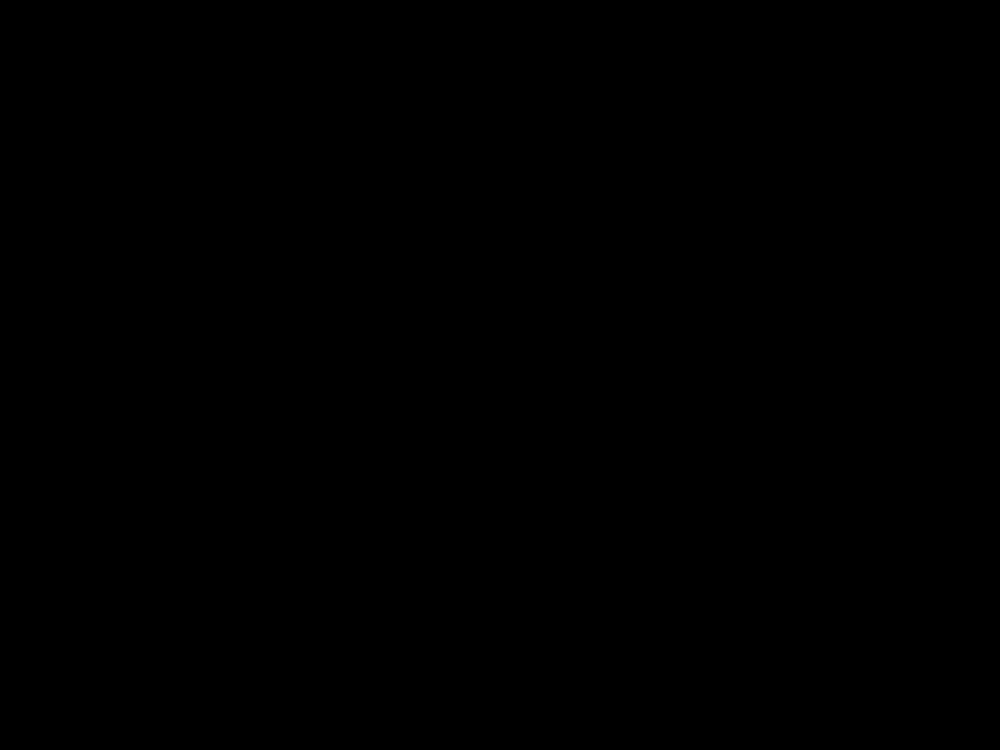
\includegraphics[width=50mm]{images/placeholder.png}}
  \caption{An example of rotating and non-rotating frames of reference. Note that $(\vec{v}_{B/A})_xyz$ appears to move along the path $\vec{r}_{B/A}$ when viewed from a rotating frame of reference. When this same motion is observed relative to the $XYZ$ frame of reference it will trace a motion which is spiraling.}
\end{figure}
To find the acceleration of a rotating frame of reference we take the time derrivative of equation (17). this looks as follows:
\begin{equation}
  \vec{a}_B = \vec{a}_A + \vec{\dot{\Omega}} \times \vec{r}_{B/A} + \vec{\Omega} \times \vec{\dot{r}}_{B/A} + (\vec{\dot{v}}_{B/A})_xyz\\
\end{equation}
where:
\begin{gather*}
  \vec{\dot{r}}_{B/A} = \vec{\Omega} \times \vec{r}_{B/A} + (\vec{v}_{B/A})_{xyz}\\
  (\vec{\dot{v}}_B/A)_{xyz} = (\vec{a}_{B/A})_{xyz} + \vec{\Omega} \times (\vec{v}_{B/A})_{xyz}
\end{gather*}
Which gives the following equation for the acceleration of $B$:
\begin{equation}
  \vec{a}_B = \vec{a}_A + \vec{\dot{\Omega}} \times \vec{r}_{B/A} + \vec{\Omega} \times (\vec{\Omega} \times \vec{r}_{B/A}) + 2\vec{\Omega} \times (\vec{v}_{B/A})_{xyz} + (\vec{a}_{B/A})_{xyz}
\end{equation}
Where the term $(\vec{a}_{B/A})_{xyz}$ is the local acceleration of $B$ relative to the $xyz$ frame of reference and the term $2\vec{\Omega} \times (\vec{v}_{B/A})_{xyz}$ is the mathimatical description of the coriolis effect.

\end{document}